enü% !TEX root = ../Projektdokumentation.tex
\section{Analysephase} 
\label{sec:Analysephase}

Für die Erstellung von \acs{UML}-Diagrammen zu Analysezwecken wird sich an \cite{UML} orientiert. Die Erstellung an sich erfolgt mit dem kostenlosen Online-Programm \textit{draw.io} \footnote{\url{https://www.draw.io/}}.

\subsection{Ist-Analyse} 
\label{sec:IstAnalyse}
Derzeit haben Mieter eines ePages-Onlineshops die Möglichkeit im \acs{MBO} ihres Onlineshops, in dem alle wichtigen Shopeinstellungen zu treffen sind, zwei Analysewidgets auszuwählen, siehe \Abbildung{dashboard} Das erste zeigt eine Top-3-Liste der meistverkauften Artikel der letzten 30 Tage an und das zweite den Nettoumsatz sowie die Anzahl der Bestellungen für heute, gestern, diese Woche, letzte Woche, diesen und letzten Monat an.
\begin{figure}[htb]
\begin{center}
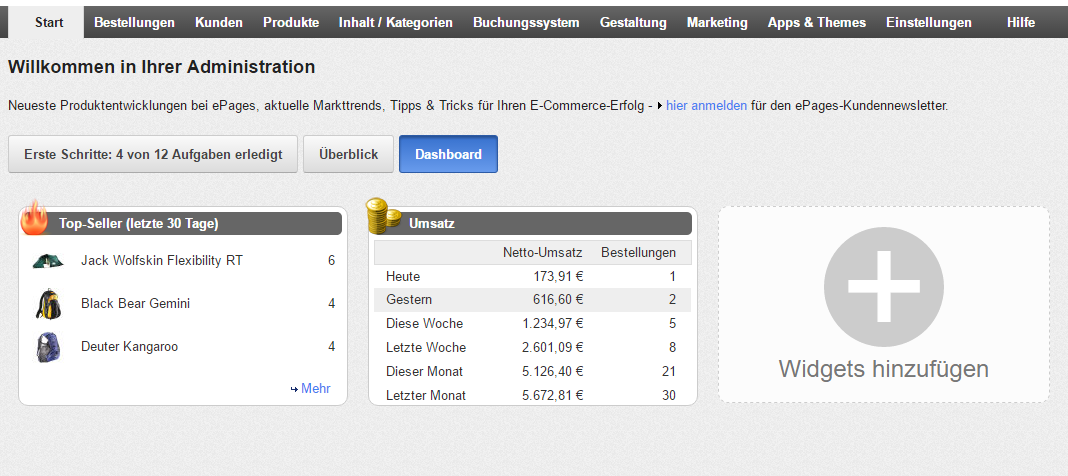
\includegraphics[width=0.9\textwidth]{dashboard.png}
\caption{Widgetauswahl im Dashboard des \acs{MBO}s eines ePages Onlineshops}
\label{fig:dashboard}
\end{center}
\end{figure}
Des Weiteren wurde bereits auf einem zweitägigen firmeninternen Hackathon im Frühjahr 2016 der Versuch der Programmierung einer Statistik-App unternommen, wobei dabei nur mit \gqq{\acs{Mock}-Daten}  hantiert wurde und keine echte Shopanbindung realisiert wurde. Die Ergebnisse zu dieser App sind auf einer internen Wikiseite veröffentlicht und liefern einen ersten Eindruck wie so eine App aussehen könnte und welche Funktionalitäten und Use-Cases ePages vorrangig für solch eine Statistik-App vorsieht. Zu sehen ist ein Menü, über das Bestellungs- und Artikelstatistiken anwählbar sind. In \Abbildung{order} sieht man wie eine graphische Darstellung von Umsätzen pro Bestellung aussehen könnte.

\begin{figure}[htb]
\begin{center}
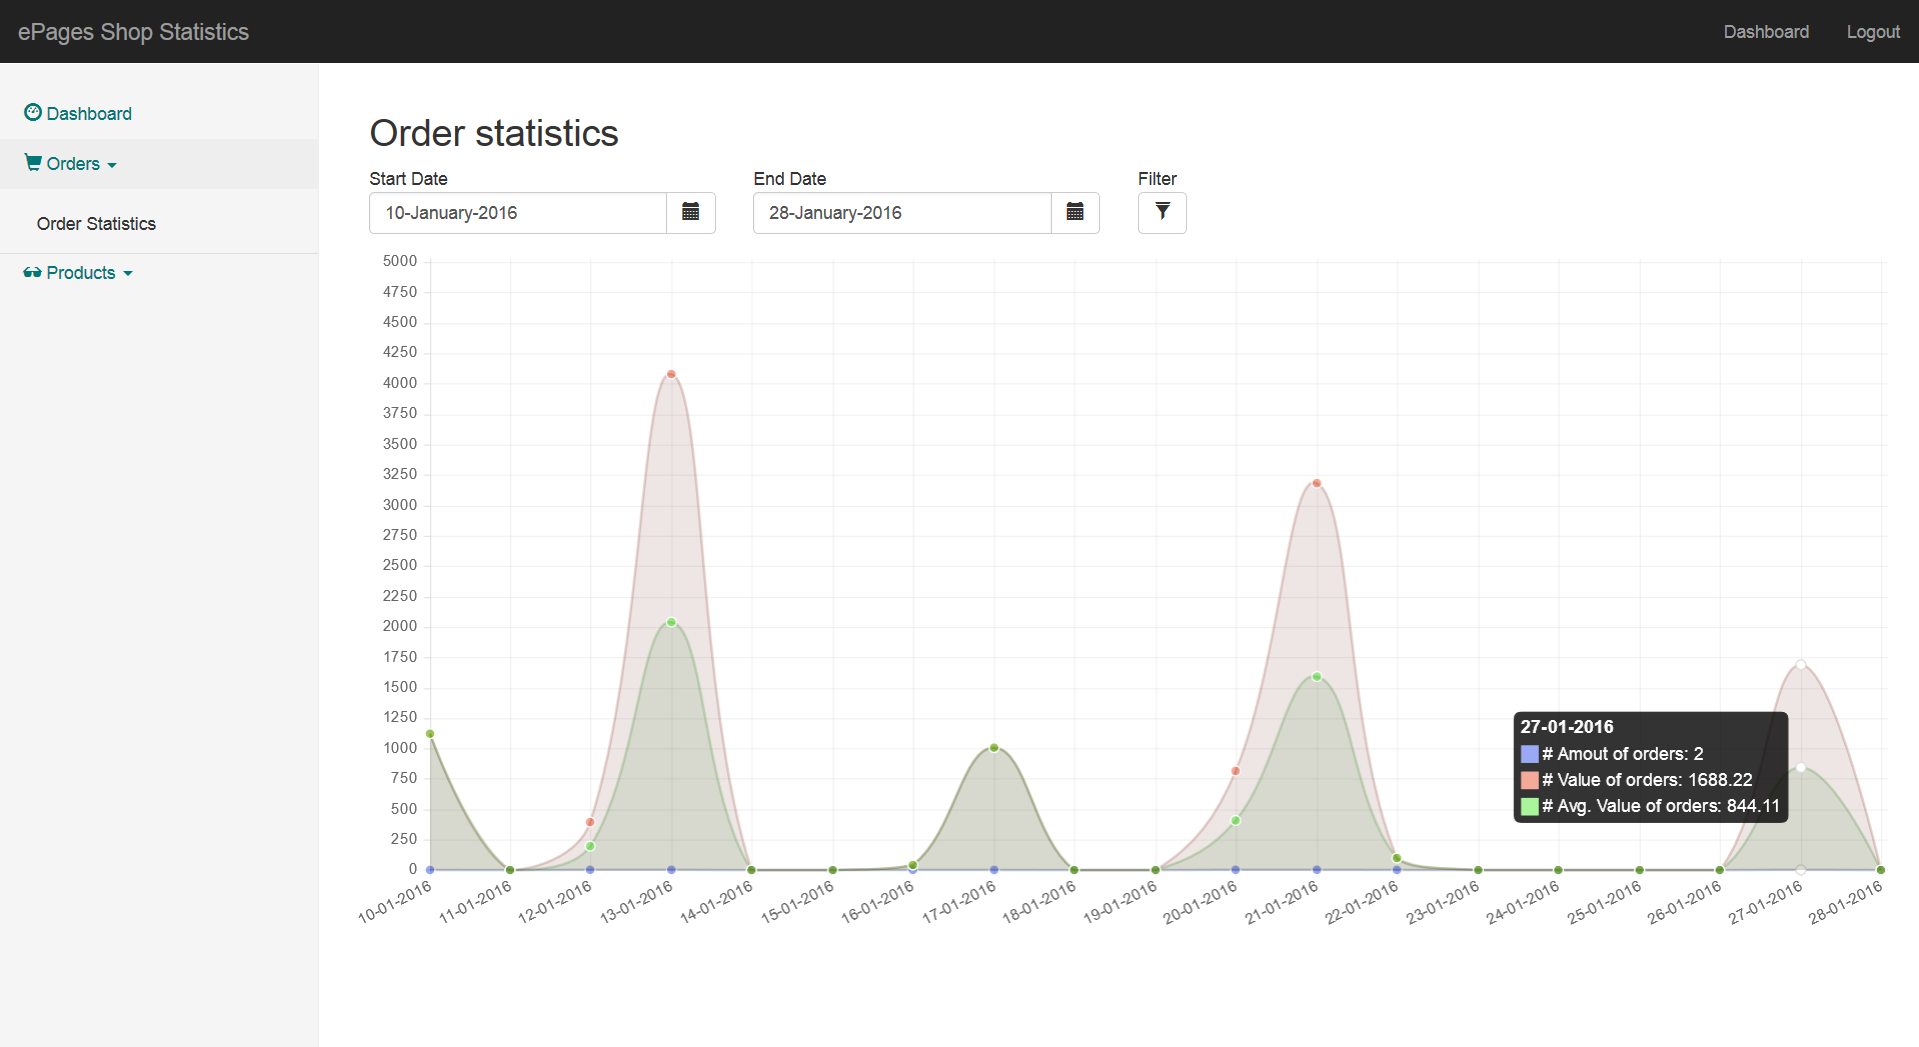
\includegraphics[width=0.7\textwidth, scale=0.5]{epagesapp1.png}
\caption{Graphische Darstellung von Bestellstatistiken}
\label{fig:order}
\end{center}
\end{figure}

\newpage

In \Abbildung{product} werden Artikel mit Gesamtumsatz und Bestellanzahl aufgelistet. Diese Beispiel-App verwendet für das Frontend das AngularJS-Framework \footnote{\url{https://angularjs.org/}} und die Backendskripte sind in Ruby on Rails programmiert. Datenbankanfragen oder angelegte Datenbanken gibt es keine, genauso wenig eine Registrierungs- oder Loginfunktionalität.

\begin{figure}[htb]
\begin{center}
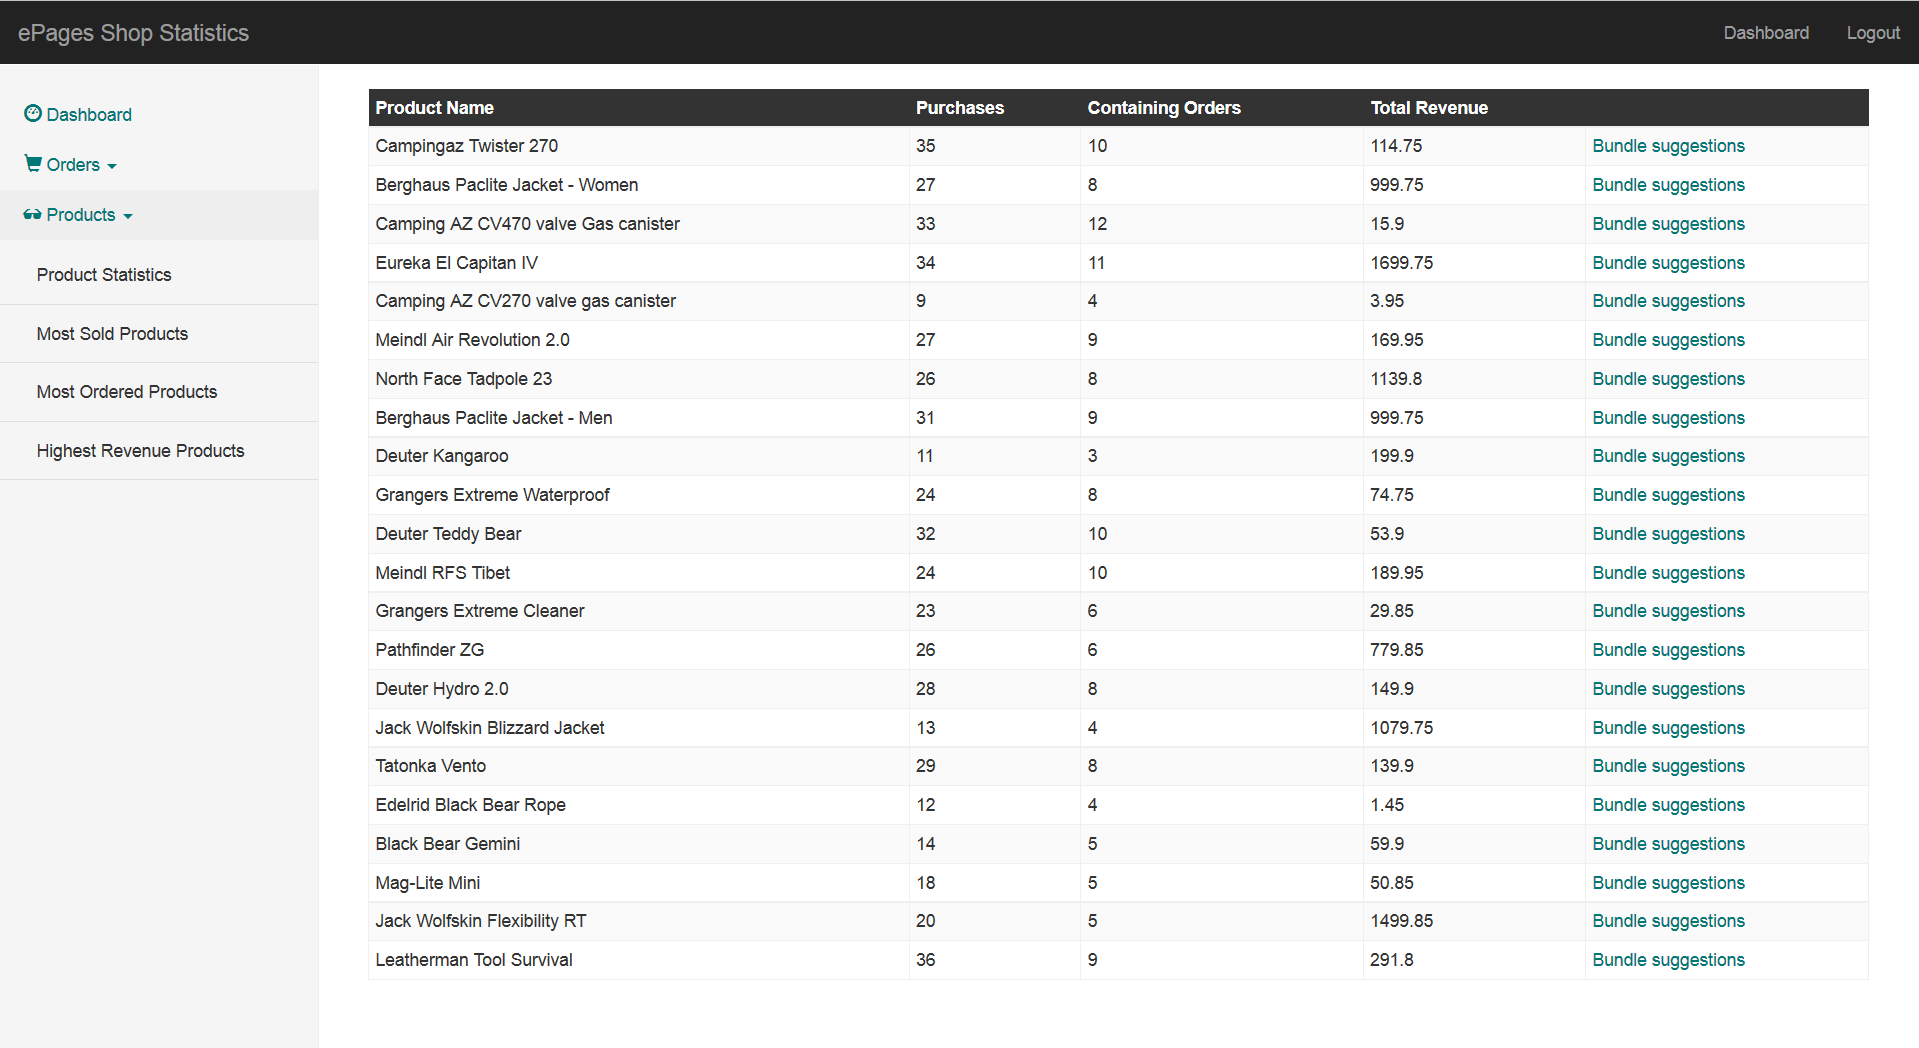
\includegraphics[width=0.7\textwidth, scale=0.5]{epagesapp2.png}
\caption{Auflistung von Artikelstatistiken}
\label{fig:product}
\end{center}
\end{figure}
 
\subsection{Wirtschaftlichkeitsanalyse}
\label{sec:Wirtschaftlichkeitsanalyse}

\subsubsection{\gqq{Make or Buy}-Entscheidung}
\label{sec:MakeOrBuyEntscheidung}

Abgesehen von den im \acs{MBO} hinzufügbaren Statistik-Wigdets
fehlen tiefergehende statistische Analysen und grafische Darstellungen der wichtigsten und interessantesten KPIs, die sich dynamisch über REST-Calls aktualisieren lassen. Darunter fallen die Möglichkeit der Berichterstattung von KPIs pro Kunde und genauere Analysen des Käuferverhaltens (Kaufabbruchrate, Herkunft, Bestellzeiten etc.). Der Wunsch nach einer auf das ePages-System zugeschnittenen App für den ePages-App-Store wurde direkt vom Produktmanagement geäußert und sollte bereits schon mal während eines zweitägigen Hackathons entwickelt werden, was jedoch aufgrund des zu hohem Zeitaufwands für die Entwicklung bei weitem nicht fertig gestellt werden konnte. Durch diese App verspricht sich das Produktmanagement eine höhere Kundenzufriedenheit und damit eine bessere Kundenbindung an die ePages Softwareprodukte sowie längerfristig eine Anwerbung neuer Kunden, die sich durch die Existenz dieser speziellen App vorzugsweise für ePages anstatt für eine andere Onlineshopsoftware entscheiden würden.
\subsubsection{Projektkosten}
\label{sec:Projektkosten}

Die Kosten für die Durchführung des Projektes setzen sich für die 70 Stunden Bearbeitungszeit sowie aus Personal- als auch Ressourcenkosten zusammen.

\paragraph{Berechnung der Entwicklungskosten für ePages}
Laut Arbeitsvertrag liegt meine Ausbildungsvergütung im aktuellen Lehrjahr bei \eur{680} pro Monat. Damit verursache ich der Firma jährliche Kosten in Höhe von 

\begin{equation}
	\eur{680}/\mbox{Monat} \cdot 12 \mbox{Monate/Jahr} = \eur{8160}/\mbox{Jahr}.
\end{equation}

Die Anzahl der Arbeitstage 2016 belaufen sich auf 252 Tage in Thüringen (Jena). Davon stehen mir 25 Urlaubstage zu. Es verbleiben (252 - 25) Tage = 227 Tage vollwertige  achtstündige Arbeitstage. Meine Stundenlohn berechnet sich damit zu

\begin{eqnarray}
	8 \mbox{ h/Tag} \cdot 227 \mbox{ Tage/Jahr} = 1816 \mbox{ h/Jahr} .\\
	\frac{\eur{8160} \mbox{/Jahr}}{1816 \mbox{ h/Jahr}} \approx \eur{4,49}\mbox{/h}.
\end{eqnarray}

Für die Nutzung der Ressourcen\footnote{Laptop, Monitore, Servernutzung, Büro- und Firmenräumlichkeiten, Stromverbrauch, Heizkosten etc.} wird ein pauschaler Stundensatz von \eur{15} angenommen. Für die anderen Mitarbeiter wird pauschal ein Stundenlohn von \eur{25} angenommen. Eine Aufstellung der Kosten befindet sich in Tabelle~\ref{tab:Kostenaufstellung} und sie betragen insgesamt \eur{1844,30}.
\tabelle{Kostenaufstellung}{tab:Kostenaufstellung}{Kostenaufstellung.tex}

\subsubsection{Amortisationsdauer}
\label{sec:Amortisationsdauer}

Geplant ist die fertige App den Nutzern der ePages-Software zur monatlichen Miete zur Verfügung zu stellen. Der Mietpreis wird in dem Bereich $[\mbox{\eur{5}},\mbox{\eur{50}}]$ liegen. Die angenommene Zahl an Nutzern liegt in dem Bereich $[\mbox{1},\mbox{20000}]$.

\paragraph{Berechnung der Amortisationszeit}
Für den Umsatz (=$U$), die diese App abhängig von der Zeit in Monaten (=$t_m$), den Nutzern (=$N$) und von dem Mietpreis pro Monat (=$p_m$) erwirtschaften soll wird die Formel $U = p_m \cdot N \cdot t_m$ zugrunde gelegt. Es wird angenommen, dass die App nach einem Monat 10 Nutzer hat. Dieser Wert wird modellhaft als linear ansteigend mit der Zeit $t_m$ angenommen, d.h. $N = 10 \cdot t_m$. Daraus lässt eine Formel zur Berechnung der Amortisationszeit ($t^{A}_m$) ableiten:

\begin{eqnarray}
	t^{A}_m &=& \frac{U}{p_m \cdot N},\quad \mbox{wobei}\quad U = \mbox{\eur{1844,30},}\quad N = 10 \cdot t_m^{A}\\
	\Rightarrow t^{A}_m &=& \sqrt{\frac{\eur{1844,30}}{10 \cdot p_m}} = 13,58 \cdot p_m^{-\frac{1}{2}}.
\end{eqnarray}

Aus dem Funktionsgraphen aus \Abbildung{AM} lässt sich die Amortisationszeit $t_m^{A}$ für jeden möglichen Mietpreis pro Monat ablesen, wobei die Unsicherheit über das Ergebnis bei kleinen Monatsmietpreisen am geringsten ist, so liegt beispielsweise die Amortisationszeit für \eur{5} Monatsmiete bei ca. 6 Monaten, was durchaus im akzeptablen Budget- bzw. Investitionsrahmen der Firma ist.

\begin{figure}[htb]
\centering
\includegraphicsKeepAspectRatio{graph.png}{0.6}
\caption{Amortisationszeit pro monatlicher Miete}
\label{fig:AM}
\end{figure}

\subsection{Anwendungsfälle}
\label{sec:Anwendungsfaelle}

Die zu entwickelnde App soll die folgenden Anwendungsfälle aus für den Nutzer/Merchant dargestellt in einem Anwendungfalldiagramm \Abbildung{usecase2} mindestens 
realisiert haben.
\begin{figure}[htb]
\centering
\includegraphicsKeepAspectRatio{usecase2.png}{1.0}
\caption{Anwendungsfalldiagramm für die Statistik-App}
\label{fig:usecase2}
\end{figure}


\subsection{Qualitätsanforderungen}
\label{sec:Qualitaetsanforderungen}

Die App soll intuitiv vom Benutzer bedien- bzw. navigierbar sein. Alle dargestellten Statistiken und Berichte sollen selbsterklärend sein. Die App wird als Single-Page-Anwendung programmiert, d.h. bei keiner Aktion des Benutzer soll ein Seitenneuladen ausgelöst werden. Bei Aktualisierung der Daten durch Datenbankabfragen, wenn beispielsweise die Währung oder der Zeitraum geändert wird, sollen alle betroffenen Diagramme und Berichte nahezu gleichzeitig mit den neuen Daten aktualisiert werden. Bei der Datensynchronisation soll der Nutzer eine Rückmeldung darüber erhalten, ob die Synchronisation noch im Gange ist oder nicht oder gar fehlgeschlagen ist.

Zusätzlich soll für jeden Nutzer beim Login eine zeitlich befristete gültige Session gestartet werden, sodass die \acs{URL} für diesen Client einzigartig ist und bei keinem anderen Clientcomputer oder Browser gleichzeitig verwendet werden kann. Das Design sollte für den Nutzer ansprechend sein und die App sollte in Ansätzen \gqq{responsive} sein, um auch auf mobilen Geräten benutzbar sein zu können.
Die App soll frontend- und backendseitig modular aufgebaut sein, so dass Fehlerbeseitigung oder Modifizierungen schnell und übersichtlich möglich sind und sich konsistent in das Gesamtprogramm einfügen.
Der Programmcode sollte strukturiert nach gängigen oder firminternen Code-Conventions sein und an allen wichtigen Stellen Kommentare für Entwickler enthalten.


\subsection{Lastenheft/Fachkonzept}
\label{sec:Lastenheft}

Die Anwendung muss folgende Anforderungen erfüllen:
\begin{enumerate}
\item Registrierungsmechanismus
\begin{enumerate}
\item Der Nutzer muss Vorname, Name, Email-Adresse, Passwort und seine Shop-\acs{URL} zur Registrierung eingeben können.
\item Die Passworteingabe sollte blicksicher sein und verifiziert werden.
\item Nach der Registrierung bekommt man eine Erfolgsmeldung und wird auf die Loginseite weitergeleitet.
\end{enumerate}
\item Login-Mechanismus
\begin{enumerate}
\item Die Logindaten sollen die Email-Adresse und das Passwort sein.
\item Bei Falscheingabe von Email-Adresse oder Passwort soll eine entsprechende Rückmeldung erfolgen.
\end{enumerate}
\item Logout-Mechanismus
\begin{enumerate}
\item Im Nutzerbereich der App soll eine Möglichkeit zum Beenden der Session/Logout geschaffen werden.
\item Beim Ausloggen soll die Session beendet und eine Weiterleitung auf den Loginbereich erfolgen.
\end{enumerate}
\item Navigation im Nutzerbereich
\begin{enumerate}
\item Alle wesentlichen Benutzerinteraktionen der App sollen nur über ein einziges Navigationspanel entweder an der Seite oder oben als Leiste durchführbar sein.
\item Die Navigation sollte einen logischen und intuitiven Aufbau haben und sollte vom Design her einheitlich sein.
\end{enumerate}
\item Graphische Darstellungen statistischer Auswertungen
\begin{enumerate}
\item Die Umsätze und Bestellungen im Onlineshop sollen wahlweise als Balken- oder Liniendiagramme darstellbar sein.
\item Für die Diagramme soll der Zeitraum auswählbar über die Menüleiste sein. Die auswählbaren Zeiträume sollen mindestens die einzelnen Kalenderwochen, Monate und Jahre umfassen.
\item Es soll möglich sein, die Diagramme wahlweise aufgrund von Brutto - oder Nettoumsätzen anzuzeigen.
\end{enumerate}
\item Währungsfilter
\begin{enumerate}
\item Die Anzeige der Statistiken und Berichte sollte abhängig von der  ausgewählten Währung sein, da im Onlineshop mehrere Währungen eingestellt sein können.
\item Hierzu muss eine Auswahlmöglichkeit über einen Währungsfilter geschaffen werden.
\end{enumerate}
\item Datensynchronisation
\begin{enumerate}
\item Es soll die Möglichkeit für den Nutzer geschaffen werden über einen \gqq{Button} die Datensynchronisation zwischen seinem Shop und der App auszulösen, falls der Nutzer eine neuerliche Synchronisation für notwendig hält.
\item Der Nutzer soll eine Rückmeldung über den Prozess der Synchronisation bekommen und eine entsprechende Mitteilung falls die Synchronisation fehlgeschlagen ist.
\item Die Daten sollen über \acs{REST}-Calls unter Verwendung der ePages \acs{REST-API} vom Onlineshop angefordert und in einer \acs{MySQL}-Datenbank abgespeichert werden.
\end{enumerate}
\item Datenbank
\begin{enumerate}
\item Zum Aktualisieren der App-Statistiken durch Benutzerinteraktionen abseits der Datensynchronisation sollen keine \acs{REST}-Calls mehr ausgelöst werden, um die ePages-REST-API nicht zu sehr zu belasten. Vielmehr sollen hier die benötigten Daten aus der Datenbank abgefragt werden.
\item Es soll ein Datenbankmodell in der 3. Normalform entworfen werden.
\end{enumerate}
\item Umsatzstatistik nach Bundesland
\begin{enumerate}
\item Es soll über ein Tortendiagramm möglich sein, die Umsatzverteilung pro Bundesland angezeigt zu bekommen.
\item Außerdem sollen Shopkunden dabei berücksichtigt werden, denen kein Bundesland zugewiesen ist oder die im Ausland wohnen.
\end{enumerate}
\item Darstellung umsatzstärkster Kunden
\begin{enumerate}
\item Die App soll in tabellarischen Stil die Kunden geordnet nach Umsatz auflisten mit Namen, Email-Adresse, Gesamtumsatz, Gesamtzahl an Bestellungen und letztem Bestelldatum.
\item Die Erstellung der Tabelle sollte dynamisch erfolgen.
\end{enumerate}
\item Design
\begin{enumerate}
\item Die gesamte App sollte zumindest ein grundlegendes responsives Verhalten aufgrund des 12er-Grid-Systems zeigen.
\end{enumerate}
\end{enumerate}



